\chapter{EPCglobal Architecture Framework}

\section{Context}

Advances in \acs{uhf}~\acs{rfid} gathered a lot of attention and investment in the beginning of the decade. The technology promised, for years, a disruption in the \ac{scm} which was never delivered. 

Item level identification allows companies to capture product lifecycle information at remarkable levels of detail. \ac{rfid} readers placed through out the supply chain can automatically capture information about tagged objects while they move from manufactured to consumer.
An infrastructure that bridges the gap between the physical and the digital world, providing real-time information about current supply chain operations.
Furthermore, the instant share of information between intervening companies increases supply chain visibility, resulting in reduced uncertainty in operational and tactical supply chain planning.
Stock levels could be precisely controlled and shared with trading partners, which in turn reduces inventory costs and optimizes intra-company operations~\cite{lorenzDiscoveryServicesEPC2011, simchi-leviCadeiasSuprimentosProjeto2003}.

It was an utopia ahead of is time. The technology was not mature enough, the return on investment was not appealing and cloud computing had just started to get traction.

This did not stop the conceptualization and development of architectures capable of delivering the promises we were hoping for.
The architecture that stood relevant through out these uncertain times is the \emph{EPCglobal Architecture Framework}.
It was created and maintained by GS1, a non profit organization tasked with developing global standards for business communications.
The organization has the experience, resources and influence to make this utopia a reality.
The architecture shows on paper an appealing concept of a network capable of doing amazing thing for the \ac{scm} without restricting businesses \ac{it} architectures.

\subsection{Standardization Efforts}

Standardization of \acs{uhf}~\acs{rfid} for item level tagging and supply chain, by organizations like GS1, provided a common language to identify, capture and share supply chain data, ensuring important information is accessible, accurate and easy to understand~\cite{anonymousStandardsGS12014}.

The first prominent adoption was by the \ac{dod} with a policy released on July 30th 2004. The policy stated that contracts issued for material delivery would require the use of \ac{uhf} tags. The policy was later extended to all commodities and commodities pallets shipped to any \ac{dod} facility~\cite{DoDSuppliersPassive, DODReleasesFinal}.

In 2014, Impinj, Intel, Google and Smartrac, joined forces to create the RAIN RFID alliance after the ratification of GS1's \acs{uhf}~\acs{rfid} Generation 2 version 2 standard in November of 2013. The alliance promotes the universal adoption of GS1's Gen2 \acs{uhf}~\acs{rfid} technologies and cloud computing, where \ac{rfid}-based data can be stored, managed and shared via the Internet~\cite{WhatRAINRFID}.
The alliance fortified the adoption of GS1's standards and traced a common path for the the industry to progress~\cite{TechnologyCompaniesCreate}.

On October 11th 2018 the European Commission published their positive implementation of the upper band for European countries~\cite{302208v030101pPdf}.
It extended the power levels to $2W$ in the lower band and added the requested global band from $915$MHz to $921$MHz with power levels up to $4W$. 
This was the biggest effort by the European Commission to establish a global standardized frequency band for \acs{uhf}~\acs{rfid} supply chain applications.

\subsection{Current Problems} \label{sec:currentproblems}

There are still \ac{rfid} tags that do not conform with the international standards, often presenting proprietary formats and even encoding errors.
These closed practices and struggle for market supremacy around \acs{uhf}~\acs{rfid} creates a problematic situation that prevents conformity through the global logistics market.

Even in global standards, the adoption depends on the company and field of business. Usually one identification standard is already being used, and the migration cost for supporting multi-code integration can be high.

The information around global standards is also limited and hard to get through. It is divided in multiple specifications, identified with number notation and codification nomenclature. 
The ISO standards, in specific, are closed and have to be payed before even see it's contents.
These specifications are extensive and don't provide newcomers a good experience. 
Companies planning to implement \acs{uhf}~\acs{rfid} systems following legitimate global standardization resort to consultants who have a deep knowledge on the standards complexity.

The closed mentality in the area slowed the industry progression. In comparison with the cloud and web industries, where experience and software is shared and open-sourced, \acs{uhf}~\acs{rfid} tends to keep everything closed~\cite{WhatCouldSlow}. The existent freely available software is old, outdated and out of maintenance. Experience from real-world implementations is unavailable and it is not shared, making the industry prone to committing recurrent mistakes. This results in high investments in time and money on engineering resources that could be shared among industry leaders.

The positive implementation of the upper band frequency in Europe for global \acs{uhf}~\acs{rfid} supply chain applications is also dependent on the acceptance by each European members. In particular, Germany and Netherlands are not accepting it~\cite{EUUpperBand}. The conflict with existing adopted bands in the countries makes a global homogeneous system a challenge that will need time to be established.

\subsection{GS1 and EPCglobal}

GS1 is a nonprofit organization dedicated to the development and implementation of standards for global supply chain solutions. 
The institution mission is to manage the GS1 System of Standards, create open, global, multi-sector standards fostering good business practices.

GS1 established itself in 2005 from the \ac{ean} International, \ac{ucc} and other local organizations from the United States~\cite{PublicationLEBENSMITTELZEITUNGa}.
The organization took under its umbrella the former \acs{ean}-\acs{ucc} roles subsuming their technologies. From those technologies, it is worth mentioning: the barcode identification system (from \ac{ean}), \ac{xml} standards, \ac{edi} transaction sets and supply chain solutions~\cite{lahiriRFIDSourcebook2005}.

The new GS1 organization then adopted much more ambitious projects, developing global standards and services for business communication.
From those efforts resulted the network for the synchronization of master data \ac{gdsn}, the \ac{epc} integration for \ac{rfid}, traceability and the upstream integration of the consumer goods industry suppliers and \emph{EPCglobal Network}.

For RFID Technology to become viable in practice, an infrastructure must exist for processing and communicating EPC data. In meeting the goal of creating a common infrastructure, \ac{mit} announced Auto-ID Release $1.0$ in October 2003. At the same time, \ac{mit} entered into an exclusive licensing agreement with GS1.
In turn, GS1 established a new division called EPCglobal to implement Release $1.0$ and to conduct further development based on industry input. This put forth an initial set of standards that formed the infrastructure for \ac{epc} data. Later, Auto-ID Release $1.0$ became the starting-point for the \emph{EPCglobal Network} and Architecture Framework~\cite{GlobalRFIDValue}.

\section{Overview}
%Activities, Standards, Goals

%EPC Uniqueness, Identifiers, Decentralized Implementation, Issuing Organization
%Review text - it is from and ex subsection prior to the revision of the new index

\emph{EPCglobal Architecture Framework} is a collection of interrelated hardware, software, and data standards that interoperate with shared network services~\cite{GS1EPCglobalArchitecture}.
These services are referred to as \emph{EPCglobal Network}, a computer network used to share \ac{epc} data between trading partners.
They are operated by GS1, its delegates and others to provide automatic, real-time identification and data sharing of items both within and outside of a company~\cite{lahiriRFIDSourcebook2005}.

The framework defines information systems, interface standards and data models. This approach frees the market of \ac{it} systems to create custom business solutions. Manufacturing can have their custom business logic closed, and expose production state information to the clients through the \emph{EPCglobal Network} with the EPCglobal interface standards.

The existence of these standards promote not only the global adoption of \ac{epc}, but also the exchange of information between business partners.
Even doe the network was design primarily for \ac{rfid} \ac{epc} data sharing, the network does not exclusively runs on \ac{rfid} data carriers. The Network can also be fed \ac{epc} data through data carriers like 1D and 2D barcodes. The interoperability with the barcode was one of the most important considerations during the planning of the network~\cite{RFIDBarcodeInteroperability}.

\subsection{Activities} \label{sec:activities}

The architecture defines three core activities, all of which have a group of standards and guidelines within the \emph{EPCglobal Architecture Framework}: \emph{Physical Object Exchange}, \emph{Infrastructure for Data Capture} and \emph{Data Sharing}.
These activities are helpful in understanding the organization and scope of the framework but should not be interpreted as extremely rigid~\cite{GS1EPCglobalArchitecture}.

\subsubsection{Physical Object Exchange} 

\emph{Identify} individual physical objects - products, cases, loads, assets, return items, among others - so they can be tracked individually.
Entities in the supply chain exchange physical objects identified with \acp{epc}.
Exchange consists in operations such as shipping, receiving goods, and so on.
For many End Users, the physical objects are trade goods, but this could not be the case.
There are many other uses, like library or asset management applications~\cite{dong-yingliDesignInternetThings2016} that differ from the supply chain trade goods model, but still involve unique identification and tagging of objects. 
The architecture must be designed to ensure that when one \textit{End User} delivers a physical object to another end user, the latter will be able to determine the \ac{epc} of the physical object and interpret it properly~\cite{GS1EPCglobalArchitecture}.

\subsubsection{Infrastructure for Data Capture} 

\emph{Capture data} about the movement of physical assets and creating visibility.
In order to gather \ac{epc} data, each \emph{End User} carries out operations within its environment. That can be the creation of \ac{epc}s for new objects, follow the movements of objects by sensing their \ac{epc}s, and gather that information into systems of record within the organization~\cite{GS1EPCglobalArchitecture}. The \emph{EPCglobal Architecture Framework} defines interface standards for the major infrastructure components required to gather and record \ac{epc} data.

\subsubsection{Data Sharing} 

\emph{Exchange data} with \ac{it} applications and trading partners, to turn visibility into information and action.
\emph{End Users} benefit from the \emph{EPCglobal Architecture Framework} by sharing data with each other, increasing the visibility they have with respect to the movement of physical objects through the supply chain. 
The \emph{EPCglobal Architecture Framework} defines \ac{epc} data sharing standards, which provide a means for end users to share data about \acp{epc} within defined user groups or with the general public, and which also provide access to \emph{EPC Network Services} and other shared services that facilitate this sharing.

% image: \emph{EPCglobal Architecture Framework} activities~\cite{Architecture6framework20140414Pdf}


\subsection{Standards}

% check EPCIS standard document section 2

% This standard defines EPC tag data formats for Generation 2 tags. It defines how the EPC is encoded on the tag and how it is encoded for use in the information systems layers of the EPC Systems Network. The standard includes specific encoding schemes for EPC General Identifier (GID).

Specifications on \ac{epc} encoding are defined under the \ac{tds}~\cite{EPCTagData} in conjunction with the encoding of \acp{epc} and data in \ac{gen2} \ac{rfid} tags.

\begin{table}[]
    \begin{adjustwidth}{-0.09\textwidth}{0em}
    \begin{tabular}{|l|l|l|}
    \hline
    \textbf{Activity}                                                                       & \textbf{Standard}                                                                                                                                           & \textbf{Status}                                                                                                                                                                                                                \\ \hline
    Object Exchange                                                       & \emph{\acs{uhf} Gen 2 Tag Air Interface}                                                                                                          & Ratified Jul 2018 v2.1.0~\cite{UHFGen2Tag}                                                                                                                                                                        \\ \cline{2-3} 
                                                                                            & \acs{hf} Class 1 Tag Air Interface                                                                                                         & Ratified Sep 2011 v2.0.3~\cite{HFClassTag}                                                                                                                                                                        \\ \cline{2-3} 
                                                                                            & \emph{\acs{epc} Tag Data Standard (\acs{tds})}                                                                                               & Ratified Nov 2019 v1.13~\cite{EPCTagData}                                                                                                                                               \\ \cline{1-1}
    \begin{tabular}[c]{@{}l@{}}Data Capture \\ Infrastructure\end{tabular} &                                                                                                                                                             &                                                                                                                                                                                                                                \\ \cline{2-3} 
                                                                                            & \emph{Low Level Reader Protocol (\acs{llrp})}                                                                                                     & Ratified Oct 2010 v1.1~\cite{LowLevelReader}                                                                                                                                                             \\ \cline{2-3} 
                                                                                            & Reader Management (\acs{rm})                                                                                                               & Ratified May 2007 v1.0.1~\cite{ReaderManagementRM}                                                                                                                                                       \\ \cline{2-3} 
                                                                                            & \begin{tabular}[c]{@{}l@{}}Discovery, Configuration, and \\ Initialization (\acs{dci}) for Reader Operations\end{tabular}                  & Ratified Jun 2009 v1.0~\cite{DiscoveryConfigurationInitialization}                                                                                                                                       \\ \cline{2-3} 
                                                                                            & \emph{Tag Data Translation (\acs{tdt})}                                                                                                           & Ratified Oct 2011 v.1.6~\cite{tdtTagDataTranslation}                                                                                                                                                     \\ \cline{2-3} 
                                                                                            & \emph{Application Level Events (\acs{tds})}                                                                                                       & Ratified March 2009 v1.1.1~\cite{ApplicationLevelEvents, ApplicationLevelEventsa}                                                                                                                        \\ \cline{2-3} 
                                                                                            & \emph{\acs{epcis} Capture Interface}                                                                                                              & \acs{epcis} Ratified                                                                                                                                                                                                                 \\ \cline{2-3} 
                                                                                            & \begin{tabular}[c]{@{}l@{}}\emph{\acs{epcis} Data Standard}\\ \emph{Core Business Vocabulary (\acs{cbv})}\end{tabular} & \begin{tabular}[c]{@{}l@{}}\acs{epcis} Ratified Sep 2016 v1.2~\cite{InformationServicesEPCIS}\\ \acs{cbv} Ratified Oct 2017 v1.2.2~\cite{CoreBusinessVocabulary}\end{tabular} \\ \cline{1-1}
    Data Sharing                                                           &                                                                                                                                                             &                                                                                                                                                                                                                                \\ \cline{2-3} 
                                                                                            & \emph{\acs{epcis} Query Interface}                                                                                                                & \acs{epcis} Ratified Sep 2016 v1.2~\cite{InformationServicesEPCIS}                                                                                                                                             \\ \cline{2-3} 
                                                                                            & Pedigree Standard                                                                                                                                           & Ratified Jan 2007 v1.0~\cite{PedigreeStandardV1}                                                                                                                                                         \\ \cline{2-3} 
                                                                                            & EPCglobal Certificate Profile                                                                                                                               & Ratified Jun 2010 v2.0~\cite{EPCglobalCertificateProfile}                                                                                                                                                \\ \cline{2-3} 
                                                                                            & Object Name Service (\acs{ons})                                                                                                            & Ratified Jan 2013 v2.0.1 ~\cite{deanGS1ObjectName}                                                                                                                                                       \\ \cline{2-3} 
                                                                                            & Global Data Synchronisation Network (\acs{gdsn})                                                                                           & Ratified Nov 2020 v3.1.14~\cite{joe.horwoodGDSNStandardsMaintenance}                                                                                                                                     \\ \cline{2-3} 
                                                                                            & \begin{tabular}[c]{@{}l@{}}Lightweigh Verificationt Messaging \\ Standard\end{tabular}                                                                      & Ratified Jul 2019 v1.1~\cite{david.buckleyGS1LightweightVerification2019}                                                                                                                                               \\ \cline{2-3} 
                                                                                            & GS1 EDI~\cite{anonymousGS1ElectronicData2014}: \acs{xml} standards                                                   & Ratified Nov 2019 v3.4.1~\cite{david.buckleyGS1XMLStandards2019}                                                                                                                                         \\ \cline{2-3} 
                                                                                            & Discovery Services                                                                                                                                          & In Development                                                                                                                                                                                                                 \\ \hline
    \end{tabular}
    \end{adjustwidth}
    \caption{Standards within the EPCglobal Architecture Framework} 
    \label{tab:standards}
\end{table}

\begin{figure}[!ht]
    \centering
    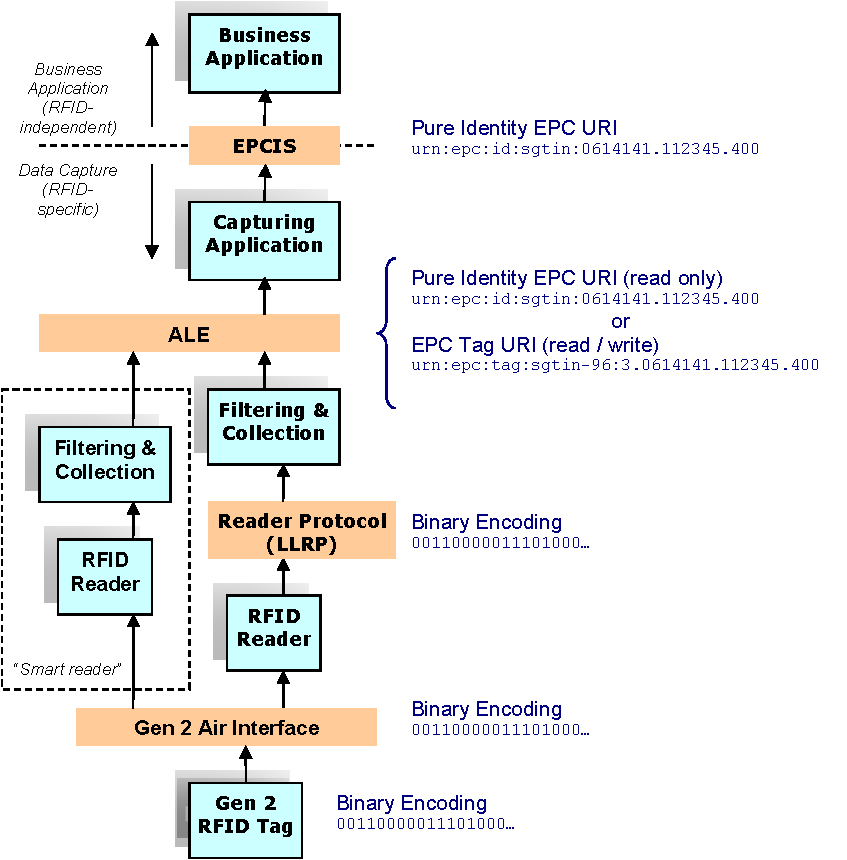
\includegraphics[width=\textwidth]{./figs/02-state-of-the-art/architecturer_structure.pdf}
    \caption{EPCglobal Architecture Framework and EPC Structures Used at Each Level~\cite{EPCTagData}} 
    \label{fig:archstructure}
\end{figure}

\section{Generation 2 \ac{uhf} Tag}

\ac{gen2} \ac{rfid} tags are passive \ac{rfid} tags that conform to the \ac{epc} Class-1 Generation-2 \ac{uhf} \ac{rfid} Standard for communications in the $860$ MHz to $960$ MHz frequency band, the ISO/IEC 18000-6 standard (Type C), or related standards currently under development.

The \ac{epc} \acl{gen2} Air Interface Protocol defines the physical and logical requirements for \ac{rfid} readers and passive tags, operating in the \ac{uhf} band, to communicate with each others~\cite{UHFGen2Tag}.
In the context of this dissertation, we are particularly interested in Class 1 \ac{uhf} tags. \ac{c1g2} tags are characterized for operating in the \ac{uhf} or \ac{hf}~\cite{HFClassTag} bands, in \ac{worm} type \ac{rfid} systems like \ac{scm} and logistics.
They are cheap, robust, support cryptographic authentication for anti-counterfeiting, functions for traceability protection and most important, are conformable with the ISO/IEC 18000-6 Type C air protocol, conjugating the two most prominent standards in \ac{uhf} conformable communication standard of operation.

It is important to address the \ac{c1g2} and ISO/IEC 18000-6 conformability. Despite the interrogation commands and logical memory map being the same, the standards differ in the data encoding. 
GS1 and ISO have different formats and encoding rules to represent \acp{id}.
Systems that want to support both encoding types have to implement interoperability between them~\cite{mizutaniMulticodePortableRFID2016a}.
In this dissertation we focus on the \emph{EPCGlobal Architecture Framework}. ISO encoding will not be covered.

\subsection{Memory}

Figure~\ref{fig:logicalmemorymap} depicts the logical memory layout in \ac{epc} Gen2 tags. It has four banks of non-volatile memory: \emph{Reserved Memory}, \emph{\ac{epc} Memory}, \emph{\ac{tid} Memory} and \emph{User Memory}. Banks can be accessed by multiples of 16 bits words.

\begin{figure}[!ht]
    \centering
    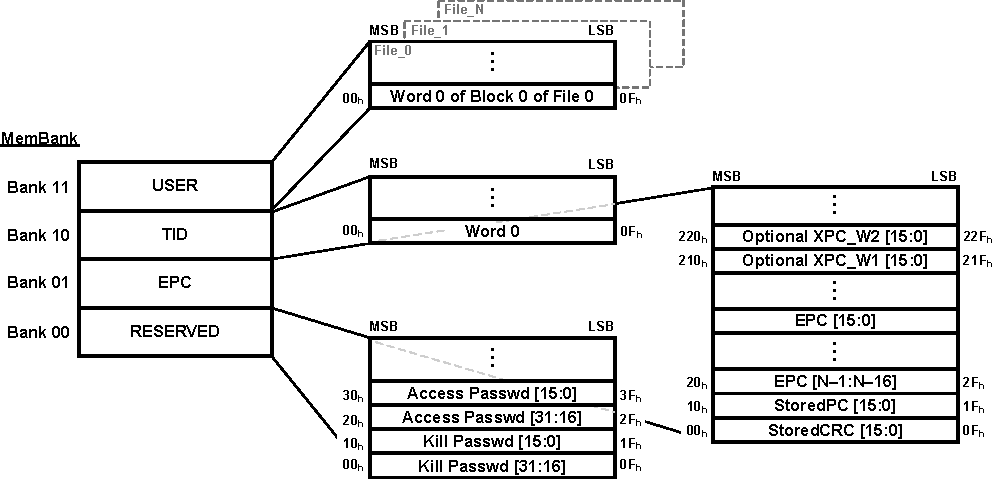
\includegraphics[width=\textwidth]{./figs/02-state-of-the-art/logicmemorymap.pdf}
    \caption{Logical memory map of EPCGlobal \ac{gen2} \ac{uhf} tags~\cite{UHFGen2Tag}} 
    \label{fig:logicalmemorymap}
\end{figure}

\subsubsection{Reserved Memory}

Reserved Memory (Bank $00$) holds the Access and Kill passwords, if implemented by the manufacturer of the Tag. 
The \emph{Kill password} is a 32-bit value used in the \emph{Kill Command} to render a tag non-responsive thereafter. The \emph{Kill Command} only executes if the password has been set to a value different from the default all-zero password.
The \emph{Access password} is a 32-bit value which allows a tag to transition in to the Secure state. In the Secure state all Access commands can executed, including writing to locked blocks. The default password is all zeros and must be changed if access protection is desirable~\cite{RFIDEPCGen2,UHFGen2Tag}.

\subsubsection{\ac{epc} Memory}

The \ac{epc} Memory (Bank $01$) contains a 16-bit \ac{crc} for error correction, a 16-bit \ac{pc} and a \ac{epc}.

\ac{epc} binary encoding will be further discussed in section~\ref{sec:binencoding}, it is the \ac{id} in which the \emph{EPCGlobal Framework} revolves around to identify every item in the world. The \ac{epc} is by design extensible, being that depending on the application requirements, it can be between $96$ bits and the maximum \ac{epc} size supported by the tag (some tags can have \ac{epc} memory up to $496$ bits). Important to refer, tag cost rises with the amount of \ac{epc} bits. Companies planning on implementing \ac{epc} must devise a serialization plan where a estimate of serial numbers and unique products is done. This will influence the requirements in \ac{epc} memory and consequently tag price.
The encoding of \ac{epc} is not defined in the \ac{gen2} air protocol standard, but in the \emph{\ac{epc} Tag Data Standard} which will be further discussed with detail on section~\ref{sec:epc}.

The standard also defines \ac{xpc} words, \acs{xpc}\_W1 and \acs{xpc}\_W2 respectively. These words are optional and usually not implemented by tag manufacturers. In fact, the tags used in this dissertation - with \textit{Impinj's Monza} chips - are widely used in all kinds of tag applications around the globe, and don't implement \ac{xpc} words. These words contain bit indicators for settings like hazardous materials and intractability to say a few.

The \ac{pc} word contains metadata used to interpret the \ac{epc}. A more detailed representation of the \ac{pc} can be seen in table~\ref{tab:pcbits}.
From $10_h-14_h$, 4 bits with the length of the \ac{epc}/\ac{id} in words, at $15_h$ a toggle bit called \ac{umi} which indicates if \emph{User Bank $11$} has any data in it, and at $16_h$ a toggle bit to indicate if the tag has extended \ac{pc}.
To distinguish an GS1 from an ISO standard \ac{id}, the most reasonable way is to look at bit $17_h$, which contains a toggle bit to indicate whether the \ac{id} is GS1 or non-GS1 family.
From bit $18_h$ to $1F_h$ is reserved for future use under the \emph{EPCGlobal} specification. Under some circumstances GS1 EPCglobal may permit other standard body or organization to use one or more of these RFU values for standardization purposes. Also to note, on ISO 18000-6, these bits are used for \ac{id}'s supplementary meta data called Application Family Identifier.

\begin{table}
    \centering
    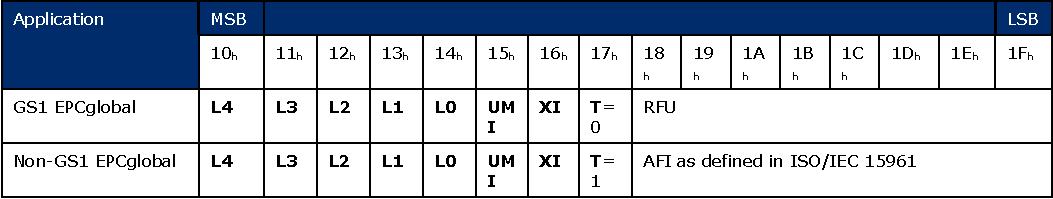
\includegraphics[width=\textwidth]{./figs/02-state-of-the-art/table_pcbits.pdf}
    \caption[\ac{pc} assignments from \ac{epc} \ac{uhf} \ac{gen2} Air Interface Protocol]{\ac{pc} assignments from \ac{epc} \ac{uhf} \ac{gen2} Air Interface Protocol~\cite{UHFGen2Tag}} 
    \label{tab:pcbits}
\end{table}

\subsubsection{TID Memory}

\ac{tid} Memory (Bank $10$) holds chip manufactured information and tag capability indicators. This memory bank is permalocked at the time of manufacture, in that it can not be changed.

The \ac{tid} Memory bank contains two fields - \ac{mdid} and \ac{tmn} - which are commonly associated together and called \ac{tid}.
\ac{mdid} encodes the tag chip manufacturer \ac{id} which is assign by GS1 as a unique identifier.
The \ac{tmn} is attributed by the manufacturer of the chip and describes the chip identification number.

In the \ac{tds}, where the encoding of \ac{tid} is specified, it is often referred has as \emph{Short} Tag Identification, because the \ac{tid} can be extended.

The \ac{tid} extension is called \ac{xtid} and is intended to provide more information about the capabilities of tags. It adds support for serialization and information about key features implemented by the tag~\cite{EPCTagData}.
Serialization is unique number generated by the tag manufacturer and can be used to uniquely identify one tag from another.
This identifies the tag itself, rather than item it is applied to.
\ac{xtid} implementations are common among tag manufactures. So common in fact, people started referring to the \ac{mdid}, \ac{tmn} and serialization  combination has \emph{\ac{tid} number}.
The \ac{xtid} is specially useful in cases where the \ac{epc} is not serialized or invalid.
An example of a \ac{tid} memory bank with \ac{xtid} can be seen in figure~\ref{fig:tid}.

\begin{figure}
    \centering
    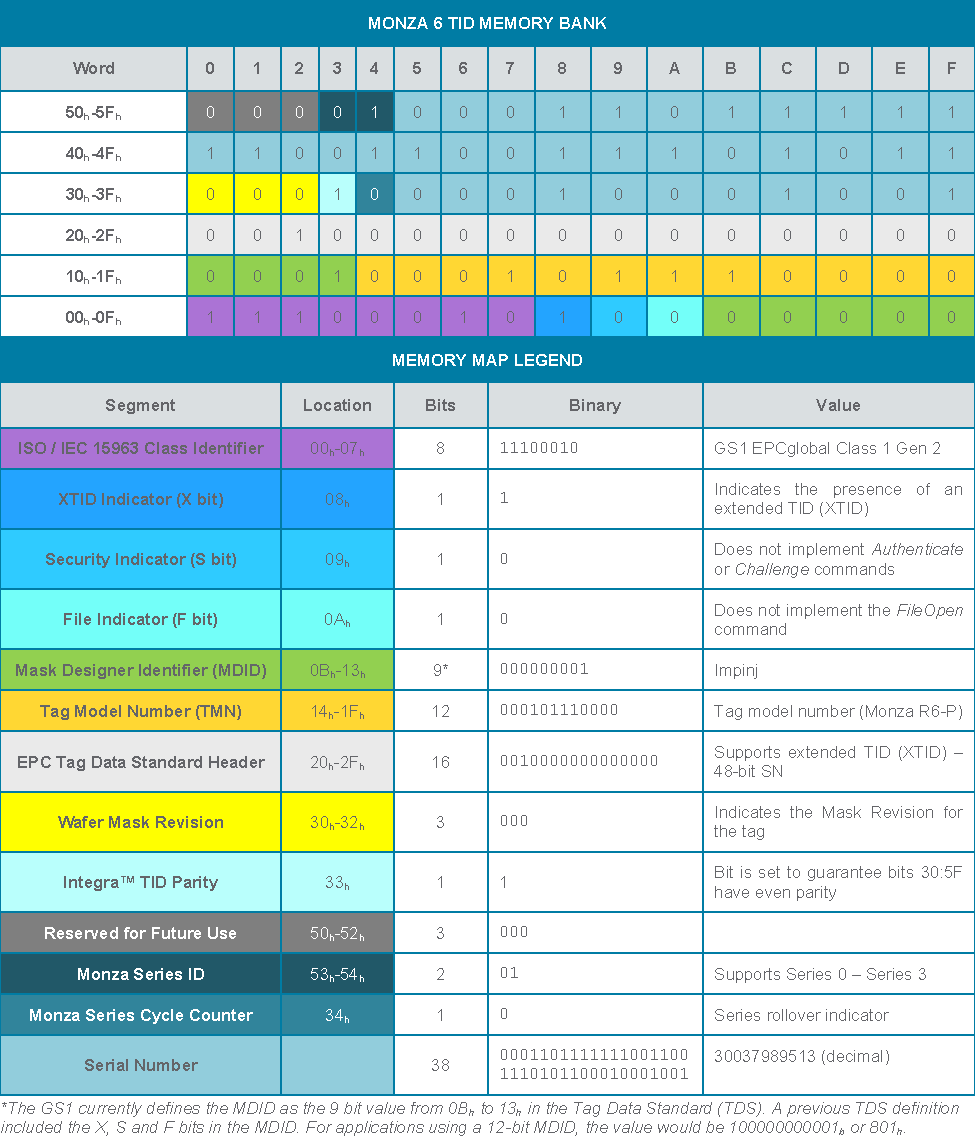
\includegraphics[width=\textwidth]{./figs/02-state-of-the-art/tid.pdf}
    \caption[\ac{tid} Memory Bank of Monza R6-P Series used in this dissertation]{\ac{tid} Memory Bank of Monza R6-P Series used in this dissertation~\cite{TIDMemoryMaps}} 
    \label{fig:tid}
\end{figure}

\subsubsection{User Memory}

The User Memory Bank provides a variable size memory to store additional data related to the tagged object.
It is frequently used to save information like temperature, maintenance logs, expiration dates and other type of data.
The bank implementation is optional and must be indicated in the \ac{umi} bit in the \ac{pc} Word.

To ensure compatibility with other protocols, the first eight bits of the bank shall contain a \ac{dsfid} as specified in ISO15962~\cite{isoISOIEC15962}.
This dissertation does not make use of the User Memory Bank, whereby it will not be covered.
For further reference, GS1 presents a solution for encoding \ac{scm} data in the User Memory Bank in the \ac{tds}~\cite{EPCTagData}.

The access to the bank is made in blocks, through the \ac{gen2} Air Protocol. The arrangement of the data in the Bank is important, as it can impact reading speeds.
GS1 provides a user memory encoder, a software which converts application data, into suitable encoded data ready to be stored in the User Memory Bank of \ac{gen2} \ac{rfid} tags~\cite{marco.santos.diamondFAQ2020}.

\section{\acf{epc}} \label{sec:epc}

% Check page 24 of the GS1 EPCglobal architecture Framework pdf

\ac{epc} is a universal identifier used to identify every physical object anywhere in the world.
Differently from common \ac{uuid} identifiers, \ac{epc} has a set of collective terms for the identification code, standardized by GS1~\cite{GS1GeneralSpecifications}. These terms convey context about the physical object in the encoding of the \ac{epc} itself.

\subsection{\ac{epc} in EPCGlobal Architecture Framework}

\acp{epc} are presented throughout the EPCGlobal Framework in various levels of abstraction. From low-level binary encoded, in \ac{gen2} \ac{rfid} tags, to text based \acp{uri} in business level applications.
The Framework presents seven representations~\footnote{binary, tag-encoding \ac{uri}, pure-identity \ac{uri}, legacy, legacy AI, element string and \ac{ons} hostname} for a single \ac{epc}. In general, only three are primarily used: \emph{Pure Identity}, \emph{Tag \ac{uri}} and \emph{Binary Encoding}.
Referring back to figure~\ref{fig:archstructure}, we observe that the three representations are used in different contexts throughout the framework.

The \emph{Pure Identity \ac{epc} \ac{uri}} format is, as the name suggests, represented in \acf{uri} format.
GS1 uses the \ac{urn} scheme with the \texttt{epc} \ac{nid} registered for the EPCglobal's \ac{epc} and related standards~\cite{meallingUniformResourceName}.
It is the most platform agnostic representation of an \ac{epc}, offering human readability and compatibility between heterogeneous systems. 

For components like middlewares, requiring more information about the \ac{epc} memory bank of \ac{gen2} \ac{rfid} tags, the \ac{tds} provides a \emph{Tag \ac{uri}} scheme.
This representation maintains the \ac{uri} representation, changing the \ac{nss} from \texttt{id} to \texttt{tag}, and adding \textit{control information} used to guide the process of data capture of \ac{rfid} tags.
This scheme preserves information regarding the \ac{epc} Memory Bank in the \ac{urn} namespaces that are usually disregarded in business applications but necessary in middleware operations.
In other words, the \emph{\ac{epc} Tag \ac{uri}} is a text equivalent of the entire \ac{epc} memory bank contents.
Examples of booth \ac{uri} representations can be seen in figure~\ref{fig:epcurirepresentation}. 

\begin{figure}[!ht]
    \centering
    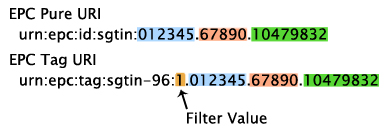
\includegraphics[width=0.7\textwidth]{./figs/02-state-of-the-art/SGTIN_First2encodings.jpg}
    \caption[\emph{Pure Identity} and \emph{Tag \acp{uri}} \ac{epc} representation]{\emph{Pure Identity} and \emph{Tag \acp{uri}} \ac{epc} representation~\cite{SGTININFO}} 
    \label{fig:epcurirepresentation}
\end{figure}

The Binary Encoding of \ac{epc} contains a compressed encoding of the EPC and additional \textit{control information} in a compact binary form, like showed on figure~\ref{fig:epcbinencoding}.
A deep analysis of the binary \ac{epc} encoding will be presented in section~\ref{sec:binencoding}.

\begin{figure}[!ht]
    \centering
    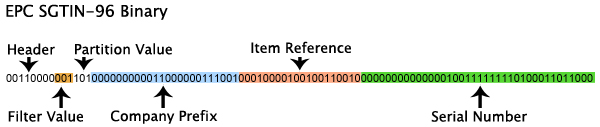
\includegraphics[width=\textwidth]{./figs/02-state-of-the-art/SGTIN_binaryconv2.jpg}
    \caption[\ac{epc} in binary encoding representation]{\ac{epc} in binary encoding representation~\cite{SGTININFO}} 
    \label{fig:epcbinencoding}
\end{figure}

\subsection{Relationship between EPCs and GS1 keys}

Before going into the encoding of \ac{epc} in \ac{gen2} \ac{rfid} tags, lets understand the underlying concepts of \ac{epc} and its schemes.

Previously, I mentioned that the \ac{epc} was designed to identify every physical object in the world.
The \emph{EPCGlobal Framework} uses this concept to its very extent.
A physical object in a \ac{scm} can be a broad term that does not provides much information regarding the object itself.
To contextualize the objects, the architecture defines GS1 keys and corresponding \ac{epc} schemes.
Each GS1 key denotes a class or grouping of physical objects. These classes encompass trade items, locations, assets, logistic units, transport groupings to say a few.
GS1 keys add valuable information to \ac{scm} operations by allowing intervening entities in the supply chain and logistics, to retrieve class context information regarding the tagged objects.

For each GS1 key there is a corresponding \ac{epc} scheme, including encoding specifications for both \ac{epc} representation: \ac{uri} and a binary encoding, for use in \ac{rfid} tags.
Each \ac{epc} scheme and corresponding GS1 key can be seen in Appendix~\ref{tab:epcschemes}.

\subsection{SGTIN}

In the scope of this dissertation, the \ac{sgtin} scheme might the most important encoding scheme to look at.
The \ac{sgtin} encodes a \ac{gtin} plus a unique product or serial number.

\begin{figure}[!ht]
    \centering
    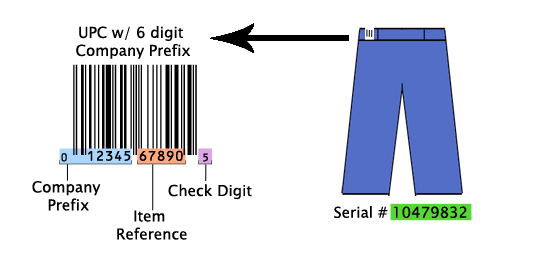
\includegraphics[width=0.8\textwidth]{./figs/02-state-of-the-art/SGTIN_UPC_Compare.jpg}
    \caption[Relation and interoperability between \ac{sgtin} and barcode's \ac{gtin}]{Relation and interoperability between \ac{sgtin} and barcode's \ac{gtin}~\cite{SGTININFO}} 
    \label{fig:barcodesgtin}
\end{figure}

The \ac{gtin} is used by companies to identify trade items~\cite{GS1GTINExecutive, GS1GTINManagement}. 
GS1 defines trade items as products or services that are priced, ordered or invoiced at any point in the supply chain.
\ac{gtin} can be used to identify types of products at any packaging level (e.g., consumer unit, inner pack, case, pallet~\footnote{even if a \ac{gtin} can be used to identify pallets, the use of \ac{sscc} is preferable~\cite{GS1KeysImplementation}}).

There are four \ac{gtin} formats: \ac{gtin}-$8$, \ac{gtin}-$12$, \ac{gtin}-$13$ and \ac{gtin}-$14$. In \ac{rfid} applications and \ac{it} applications, it is used the generalized 14-digit \ac{gtin} format. \ac{gen2} \ac{rfid} \ac{sgtin} encoding scheme is specified for \ac{gtin}-$14$.
Other \ac{gtin} formats are mainly used in barcodes in point-of-sale applications: in the \ac{us} is commonly used a \ac{gtin}-$12$ with UPC barcodes for single products and \ac{gtin}-$14$ with ITF-14 barcodes for product grouping. In contrast, in the rest of the world is commonly used \ac{gtin}-$8$ with \ac{ean}-8 barcodes for single products and \ac{gtin}-$13$ with \ac{ean}-13 for single products packaging configurations~\cite{BarcodeGS1General,GS1BarcodeChart}.

A \ac{gtin} is composed of three field: \emph{Company Prefix}, \emph{Item Reference} and check digit. All these fields are encoded in the same manner in the different N-digit \ac{gtin} formats. A \ac{gtin}-$13$ can be converted in a \ac{gtin}-$14$ by adding a leading zero, and other \acp{gtin} formats follow the same logic.

GS1 \emph{Company Prefix} is an identifier licensed by GS1 to identify a company globally. 
Nowadays, the registration of such is essential to companies wishing to sell products in big retail stores and digital marketplaces like Ebay and Amazon~\cite{ListingRequirementsProduct}).
A \emph{Company Prefix} does not uniquely identify a manufacturer. Companies can register and own more than one \emph{Company Prefix}~\cite{GS1EPCglobalArchitecture}, and in certain circumstances \emph{Company Prefixes} can change.
When licensing a \emph{Company Prefix}, there is an assessment and plan of unique product items a company shall produce. 
Depending on that, GS1 attributes a prefix with a length adjusted to company requirements. 
Companies requiring high quantities of unique item are given a shorter Company Prefix, accommodating more digits for item identification.
Also worth mentioning, the attribution of \emph{Company Prefixes} is made by one of the GS1 branches. Each branch has a prefix which uses to assign \emph{Company Prefixes} (e.g.\ GS1 Portugal has $560$, GS1 Schweiz, Suisse and Svizzera have $760$-$769$)~\cite{anonymousGS1CompanyPrefix2014}.

\emph{Item References} are assign by the managing entity of the product.
The item reference must be concatenated with the \emph{Company Prefix} to calculate the Check Digit, forming a \ac{gtin}.
From a \ac{gtin}, an \ac{sgtin} can be commissioned~\footnote{``Commisioning'' is the technical term used when creating new \acp{epc} for objects}, allowing to uniquely identify a product within its product grouping.
Important to clarify, when a \ac{gtin} is stored in \ac{rfid} tags, as in \ac{sgtin} coding schemes, the Check Digit has no purpose, so it is dropped. The Check Digit exists for error checking in barcodes. When converting barcode \ac{gtin} to \ac{epc} \ac{sgtin} encoding scheme, the Check digit must be dropped.

\subsection{Binary Encoding} \label{sec:binencoding}

Lets now understand how \acp{epc} are stored in \ac{gen2} \ac{rfid} tags.
We will focus on \ac{sgtin} encoding scheme, but the encoding method is analogous to other encoding schemes.

The binary encoding of an \ac{epc} consists of a fixed length header followed by a series of fields inherent to the encoding scheme like showed on \ac{sgtin}-$96$ Coding table~\ref{tab:sgtin96codingtable}.
For instance, lets take the \emph{Tag \ac{uri}}
\mintinline{python}{urn:epc:tag:sgtin-96:1.76300544.07470.2}
has example.
This \emph{Tag \ac{uri}} presents a \ac{sgtin}-$96$ encoding scheme, \emph{Filter value} of $``1"$, \emph{Company Prefix} $``76300544"$, \emph{Item Reference} $``7470"$ and serial $``2"$.

\begin{table}[]
    \centering
    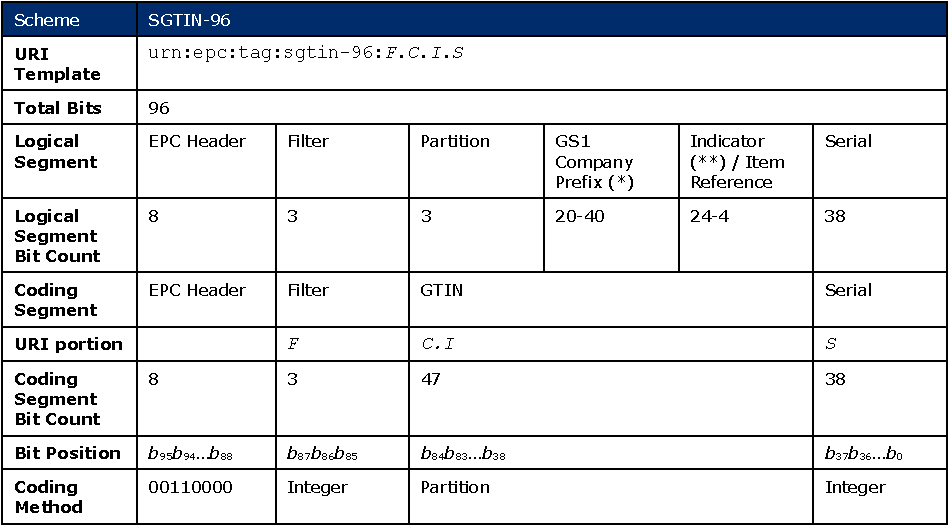
\includegraphics[width=\textwidth]{./figs/02-state-of-the-art/table_codingtable.pdf}
    \caption[Coding Table of \ac{sgtin}-$96$]{Coding Table of \ac{sgtin}-$96$~\cite{EPCTagData}} 
    \label{tab:sgtin96codingtable}
\end{table}

Following table~\ref{tab:encodingexample}, showing the \emph{Tag \ac{uri}} encoding, we first need to address the \ac{epc} header value.
A snippet of the \ac{epc} header values can be seen in table~\ref{tab:epcheaders}. We observe that an \ac{sgtin} with $96$-bit coding scheme encodes a $8$-bit header with binary value of $``00110000"$.

\begin{table}[]
    \begin{adjustwidth}{-0.00\textwidth}{0em}
    \begin{tabular}{@{}lllrl@{}}
        \toprule
        \textbf{Field}                                            & \textbf{Value (dec)} & \textbf{Value (bin)}                                                              & \textbf{\begin{tabular}[c]{@{}r@{}}Length \\ (bits)\end{tabular}} & \textbf{Notes}                                                                                                      \\ \midrule
        \ac{epc} Header                                                & 48                   & 00110000                                                                          & 8                                                                 & \ac{sgtin}-$96$ encoding                                                                                                 \\
        Filter Value                                              & 1                    & 001                                                                               & 3                                                                 & \ac{pos} item                                                                                                            \\
        Partition Value                                           & 4                    & 100                                                                               & 3                                                                 & Company Prefix has 8 digits                                                                                         \\
        \begin{tabular}[c]{@{}l@{}}Company \\ Prefix\end{tabular} & 76300544             & \begin{tabular}[c]{@{}l@{}}1001000110001000\\ 00100000000\end{tabular}            & 27                                                                &                                                                                                                     \\
        \begin{tabular}[c]{@{}l@{}}Item\\ Reference\end{tabular}  & 7470                 & 00001110100101110                                                                 & 17                                                                & \begin{tabular}[c]{@{}l@{}}Length depends on the partition\\ MSB zero fill\end{tabular}                             \\
        Serial                                                    & 2                    & \begin{tabular}[c]{@{}l@{}}0000000000000000\\ 0000000000000000000010\end{tabular} & 38                                                                & \begin{tabular}[c]{@{}l@{}}Serial is of fixed length.\\ Can be extended with \\ bigger EPC Memory Bank\end{tabular} \\ \bottomrule
        \end{tabular}
    \end{adjustwidth}
    \caption[\ac{sgtin}-$96$ binary encoding example of \mintinline{python}{urn:epc:tag:sgtin-96:1.76300544.07470.2} \emph{Tag \ac{uri}}]{\ac{sgtin}-$96$ binary encoding example of \mintinline{python}{urn:epc:tag:sgtin-96:1.76300544.07470.2} \emph{Tag \ac{uri}} retrieved from the Platform developed in this dissertation} 
    \label{tab:encodingexample}

\end{table}

\begin{table}[]
    \centering
    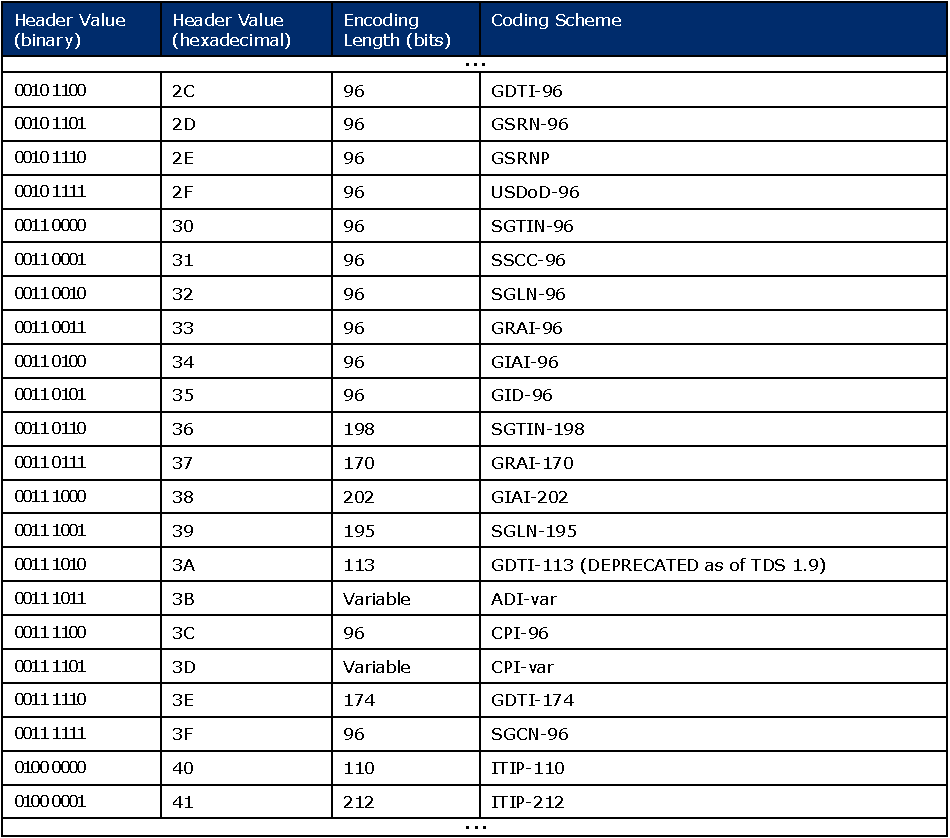
\includegraphics[width=\textwidth]{./figs/02-state-of-the-art/table_epcheaders.pdf}
    \caption[\ac{epc} headers snippet]{\ac{epc} headers snippet adapted from \ac{tds}~\cite{EPCTagData}} 
    \label{tab:epcheaders}
\end{table}

Next, we need to encode the additional \textit{information} included in the \ac{epc} Memory Bank: \emph{Filter} and \emph{Partition}. 

The \emph{Filter} encodes the packing level. An \ac{epc} \ac{sgtin} can be used to identify different levels of item packaging sharing the same \ac{gtin}. Differently from barcodes, which only encode the \ac{gtin}, an \ac{epc} with \emph{Filter} field allows a coherent \ac{gtin} across all item packages.
The \emph{Filter} value allows \ac{rfid} readers to select or deselect tags in the \emph{\ac{epc} \ac{uhf} \ac{gen2} Air Interface Protocol} corresponding to certain filter levels. This makes it easier to read desired tags in an environment where there may be other tags present (e.g.\ logistics companies only wanting to read and track Unit Loads like pallets).
Referencing table~\ref{tab:sgtinfiltervalues}, with a filter value of $``1"$, it encodes a \ac{pos} Trade Item with binary encoding of $``001"$.

The \emph{Partition} value encodes a pair of variable-length numeric fields referent to the \emph{Company Prefix} and \emph{Item Reference} memory partition. Previously we mentioned that \emph{Company Prefixes} can vary in length depending on company requirements for unique \emph{Item References}. 
In barcodes the \emph{Company Prefix} and \emph{Item Reference} are encoded together in a \ac{gtin} value. 
In \ac{gen2} tags, although there is fixed size memory shared between \emph{Company Prefix} and \emph{Item Reference}, there is also the \emph{Partition} value, which specifies the distribution of that partition between booth fields.
In the case of the \emph{Tag \ac{uri}} example, \emph{Company prefix} has $27$ bits ($8$ digits) and \emph{Item reference} has $17$ bits ($5$ digits). Referring to table~\ref{tab:partitiontable} with the pair of variable-lengths, the \emph{Partition Value} is $``4"$ encoded has $``100"$.

\begin{table}[]
    \centering
    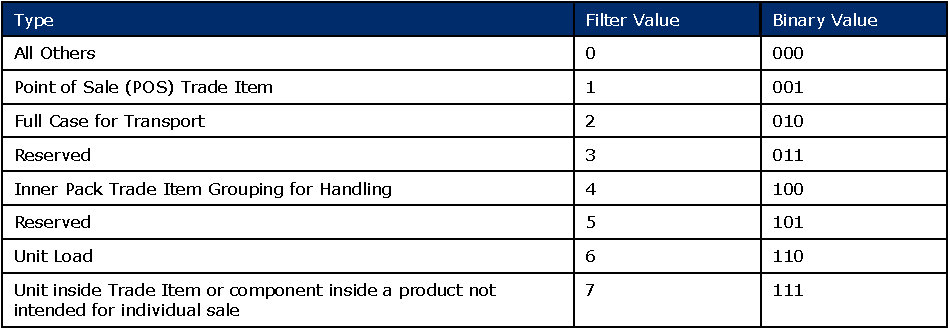
\includegraphics[width=\textwidth]{./figs/02-state-of-the-art/table_sgtin_filtervalues.pdf}
    \caption{\ac{sgtin} Filter Value Table~\cite{EPCTagData}} 
    \label{tab:sgtinfiltervalues}
\end{table}

\begin{table}[]
    \centering
    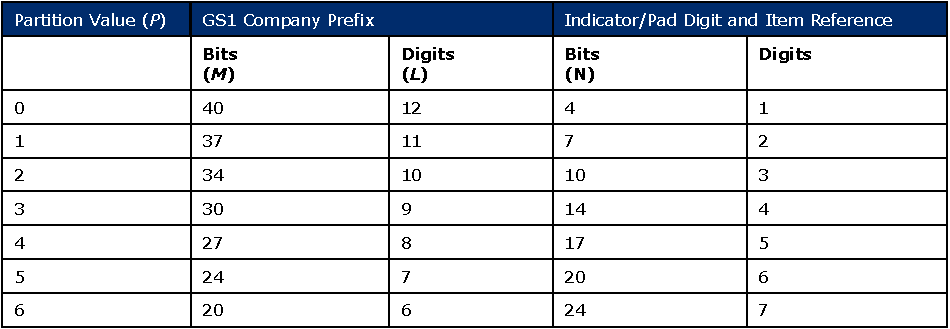
\includegraphics[width=\textwidth]{./figs/02-state-of-the-art/table_partitionvalues.pdf}
    \caption{\ac{sgtin} Partition Table~\cite{EPCTagData}} 
    \label{tab:partitiontable}
\end{table}

The \emph{Company Prefix}, \emph{Item Reference} and \emph{serial} are encoded converting from decimal to binary and add leading zeros to fill all bits in each Logical Segment.

\section{Low Level Reader Protocol (LLRP)}

The \acf{llrp} is specification for the network interface between \ac{rfid} Readers and Client applications~\cite{ImpinjLTKProgrammers}. \ac{llrp} is not exclusive to the \ac{gen2} Air Protocol. It was designed to support multiple \ac{rfid} air protocols, including future versions of \ac{gen2} Air Protocol.

\subsection{Design Requirements}

In some \ac{rfid} systems, there is a requirement for explicitly tune \ac{rfid} air protocols and the ability to control Readers that implement \ac{rfid} air protocol communications~\cite{LowLevelReader}. \ac{llrp} provides tuning features and commands for that purpose.

Devices intended to operate and communicate with \ac{rfid} Readers can vary from software applications, to middleware on local hardware, \acp{plc} and even cloud services. \ac{llrp} is ``simple'' enough to be implemented in all kinds of computer architectures.

\ac{llrp} was design without requiring real-time interaction between the application software and Reader, and but with time-critical tasks at heart. 
The Reader application software passes operational rules to the Reader in non-real time.
The Reader then triggers and runs those operation rules to achieve time-critical requirements. 
The triggers can come from the applications directly, from timers, \ac{gpi} hardware, or any other trigger defined by the Reader. 
This declarative operation method allows Readers to achieve peak performance without constraints caused by network or host latency.

\subsection{Connection Details}

\ac{llrp} is a binary protocol which runs over the \acs{tcp}/\acs{ip} internet transport protocols.
It is an asymmetric protocol where the \ac{llrp} client send commands to the Reader.

The protocol supports both reader and client initiated connections. By default, \ac{llrp} clients connect to \acs{tcp} port $5084$. In reader initiated connections, the Reader will actively try to establish a connection with the host application.
\ac{llrp} does not specify the behavior delivering data when a connection if broken. The reader used in this dissertation and others I've seen will continue to collect tag data and optionally deliver upon resumption of the connection.

Readers only allow one \ac{llrp} connection at any time. The \ac{tcp} connection between reader and client stays open until the client closes it or connection drops.

\subsection{Operation}

The primary function of the \ac{llrp} interface is to allow a client to finely tune the \ac{gen2} Tag Air Standard parameters, and command the reader to perform an inventory and otherwise access tags for read, write, lock, and kill.

To meet these requirements, \ac{llrp} defines \acp{spec}, containing descriptions of ``what, how and when'' the Reader should perform certain operations.
\acp{spec} are run when triggered. The trigger range from boundary trigger information defined in the \ac{spec} itself, \acp{gpio}, or by immediate triggers from applications for a more imperative behavior.
\acp{spec} are sent inside of messages, which are the unit of communication between client and Reader.
\ac{llrp} contains forty basic messages which range from commands, responses, events and a \textit{CUSTOM\_MESSAGE} for vender extensions. A list and description of every message can be found in Appendix~\ref{anx:llrpmessages}.

In figure~\ref{fig:ROACCESSREPORTbin} we observe an example of binary encoding of the \textit{RO\_ACCESS\_REPORT} message.
Inside the message there is a \ac{spec}, and inside a \ac{spec}, data is sent as \emph{parameters} and \emph{fields}.
\emph{Fields} are individual data elements with a known basic format.
\emph{Parameters} are named data elements that contain other parameters and/or fields, much like structures in programming languages.
Inside the \textit{RO\_ACCESS\_REPORT} message, in figure~\ref{fig:ROACCESSREPORTbin}, it can be observed the memory allocated for a list of a parameter called \textit{TagReportData}. \textit{TagReportData} is then encoded following figure~\ref{fig:TagReportDatabin}, which inside encodes an \textit{EPCData} or \textit{EPC-96} parameter, where the binary encoded \ac{epc} is allocated.
When constructing \ac{llrp} messages, parameters can be optional, but field must be presented and within their valid range. Some tooling software provides user friendly features like inferring Reader capabilities and default values for unspecified fields.

\begin{figure}[]
    \centering
    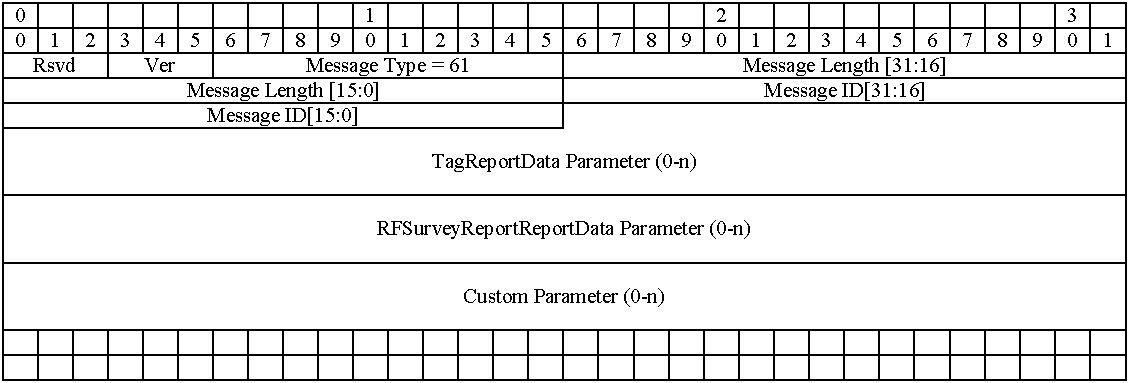
\includegraphics[width=\textwidth]{./figs/02-state-of-the-art/RO_ACCESS_REPORT_bin.pdf}
    \caption[\textit{RO\_ACCESS\_REPORT} message binary encoding]{\textit{RO\_ACCESS\_REPORT} message binary encoding~\cite{LowLevelReader}. This message is sent by the Reader and contains inventory and access operations results} 
    \label{fig:ROACCESSREPORTbin}
\end{figure}

\begin{figure}[]
    \centering
    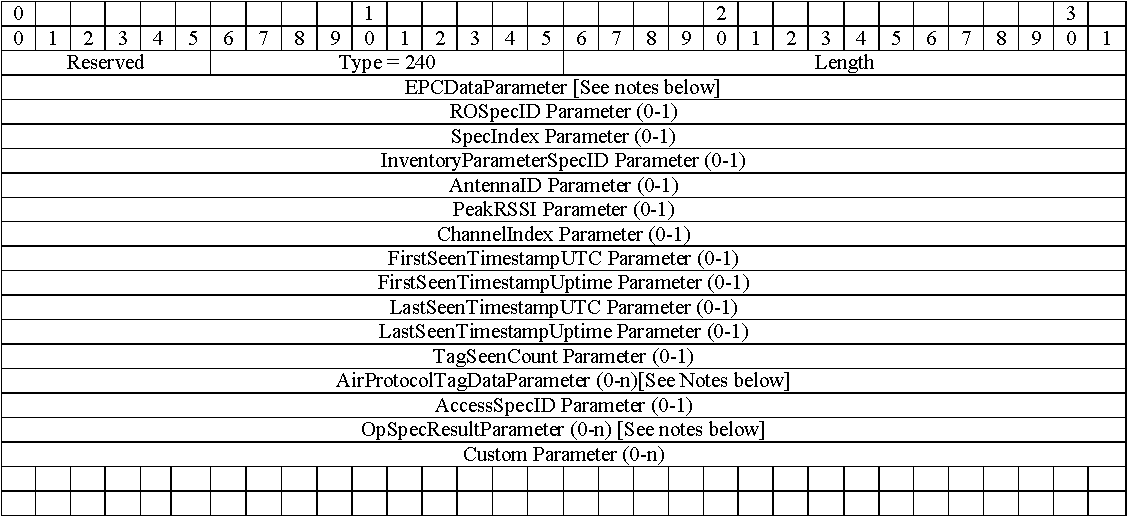
\includegraphics[width=\textwidth]{./figs/02-state-of-the-art/TagReportData_bin.pdf}
    \caption[\textit{TagReportData} parameter binary encoding]{\textit{TagReportData} parameter binary encoding~\cite{LowLevelReader}. \textit{TagReportData} is generated per tag and contains a mandatory parameter \textit{EPCData} with encoding} 
    \label{fig:TagReportDatabin}
\end{figure}

\begin{figure}[]
    \centering
    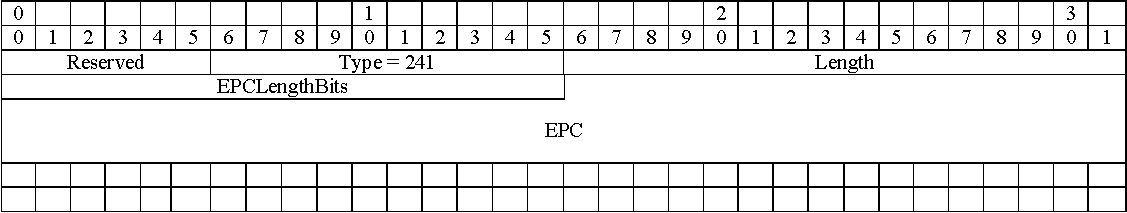
\includegraphics[width=\textwidth]{./figs/02-state-of-the-art/EPCDataParameter_bin.pdf}
    \caption[\textit{EPCData} parameter binary encoding]{\textit{EPCData} parameter binary encoding~\cite{LowLevelReader}. \textit{EPCData} shall be used for encoding a non-96 bit \ac{epc}, whereas the \textit{EPC-96} Parameter on figure~\ref{fig:EPC96bin} is be used for encoding a 96-bit \ac{epc}} 
    \label{fig:EPCDatabin}
\end{figure}

\begin{figure}[]
    \centering
    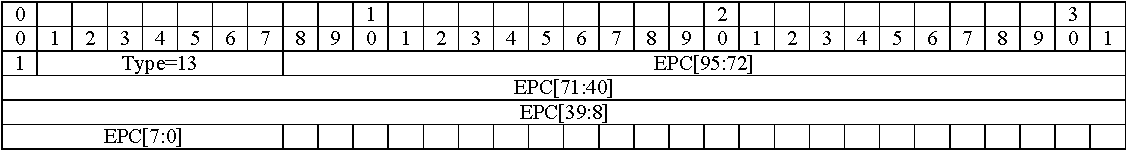
\includegraphics[width=\textwidth]{./figs/02-state-of-the-art/EPC96ParameterTVEncoding_bin.pdf}
    \caption[\textit{EPC-96} parameter binary encoding]{\textit{EPC-96} parameter binary encoding~\cite{LowLevelReader}}
    \label{fig:EPC96bin}
\end{figure}

\subsection{\acf{spec}}

There are two main \acp{spec} defined in the \ac{llrp} Standard:  \textit{\acp{rospec}} and \textit{Access \acp{spec}}. Most of other \acp{spec} and parameters are enclosed under one of the two.
I will briefly discuss relevant knowledge required to understand the \acp{spec} context. Detailed information on necessary fields will be presented later in opportune moments throughout this dissertation.

\subsubsection{\acf{rospec}}

\acp{rospec} control the operation of the Reader. They describe the inventory operations the Reader has to perform.
A Reader only supports one \ac{rospec} at a time.
An example of a \ac{rospec} is presented inside the \textit{ADD\_ROSPEC} message seen in Code~\ref{code:rospec}. \ac{xml} is used in the context of many \ac{llrp} clients to provide human readability of the binary protocol, and also used in this dissertation for the same reason.
In the \textit{ADD\_ROSPEC} \ac{xml} message we observe one \ac{rospec} and constituting parameters and fields.
\acp{rospec} contain the following elements:

\begin{description}

\item[\texttt{ROSpecID}] is an \ac{id} set by the client to uniquely identify the \ac{spec} in subsequent commands.

\item[\texttt{Priority}] should be set to $``0"$~\cite{ImpinjLTKProgrammers}. By default, all \acp{rospec} should have the same priority. High priority \acp{rospec} can preempt an active lower priority one and start execution as soon as the start condition occurs.

\item[\texttt{CurrentState}] describes the current state of the \ac{rospec} - \emph{disabled}, \emph{inactive}, \emph{active}. When adding and \ac{rospec} the state must be set to \emph{disable}.

\item[\texttt{ROBoundarySpec}] is a parameter containing a description of the start and stop conditions for the \ac{spec}. 
These conditions can be, for the start trigger:
\begin{itemize}
    \item \texttt{None/Null} - \ac{rospec} will not start unless indicated by the client application through an \textit{START\_ROSPEC} message;
    \item \texttt{Immediate} - the \ac{rospec} will start immediately after enabled, and will continuously restart itself until disabled;
    \item \texttt{Periodic} - when enabled, the \ac{rospec} will be triggered periodically;
    \item \texttt{\ac{gpi}} - the enabled \ac{rospec} will start when the \ac{gpi} event enters a certain state.
\end{itemize}

For the stop triggers:
\begin{itemize}
    \item \texttt{None/Null} - the \ac{rospec} only stops when stopped by the client through the \textit{STOP\_ROSPEC};
    \item \texttt{Duration} - \ac{rospec} stops when it has been active for a specified duration;
    \item \texttt{\ac{gpi}} - \ac{rospec} will stop when the \ac{gpi} event enters a certain state.
\end{itemize}

\item[\texttt{\ac{aispec}}] contains the settings for the Reader's antennas and \ac{gen2} Air protocol options. An \ac{rospec} can have one or more \acp{aispec} which are executed when the \ac{rospec} runs.

\item[\texttt{ROReportSpec}] is optional and describes ``when'' reports should be forward to the client and ``what'' the report contains. If not defined, the Reader will use the current or default settings.
\end{description}

\begin{listing}
    \inputminted[linenos]{xml}{./code/sota/llrp_messages/ROSPEC.xml}
    \caption{Example of \textit{ADD\_ROSPEC} message in \ac{xml} representation}
    \label{code:rospec}
\end{listing}

\subsection{Application Flow}

A typical \ac{llrp} application flow can be seen in figure~\ref{fig:llrpflow}. Upon establishing a \ac{tcp} connection, a Client add and enables an \ac{rospec}, containing information about the inventory procedures. The Client can also register a \ac{aispec} for \ac{gen2} commands, like writing \acp{epc}.
The Reader, upon trigger, executes the \acp{spec}, performing \ac{epc} inventory and tag operations, which are reported back to the Client.

\begin{figure}[!ht]
    \centering
    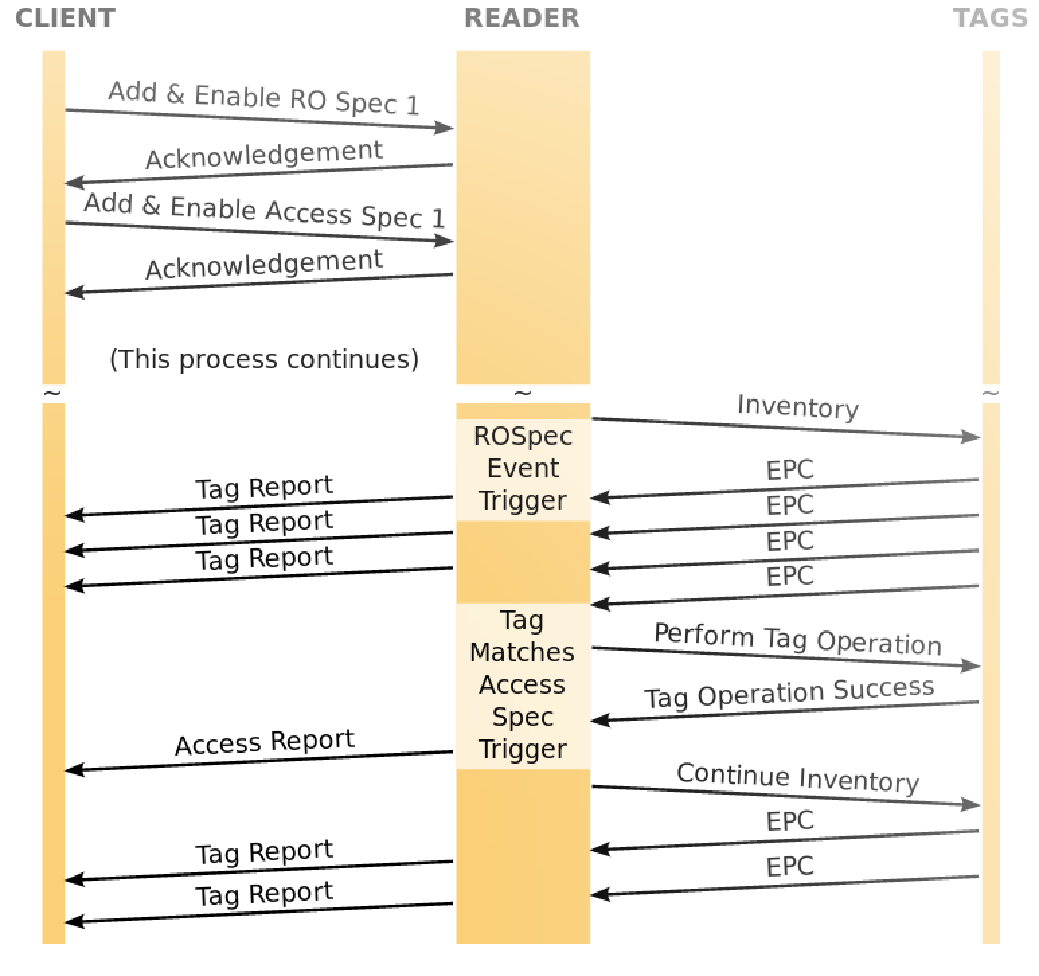
\includegraphics[width=0.9\textwidth]{./figs/02-state-of-the-art/llrpflow.pdf}
    \caption[Example of \ac{llrp} Application Flow]{Example of \ac{llrp} Application Flow~\cite{ImpinjLTKProgrammers}} 
    \label{fig:llrpflow}
\end{figure}


\subsubsection{Access \acl{spec}}

An \emph{Access \ac{spec}} handles the extended tag operations of \ac{gen2}: read, write, lock and kill.
It was design to be extensible, in order to support multiple air protocols and their respective commands.
These will not be directly used in the practical context of this dissertation, so no further description will be added.

\section{\acf{fc}}

\ac{fc} is a specification for middlewares operating between readers and client applications, to receive, filter, translate and deliver data to client applications.

\ac{gen2} \ac{rfid} readers can generate large amounts of network traffic. The amount of requests generated, containing reports with \ac{epc} raw data, can bottleneck most networks, being unsuited for internet data exchanges. 
Often, client applications are hosted in different networks and even different physical places. With the current paradigm of cloud computing, the interest in processing data on data centers only seems to be growing.
Furthermost, raw \ac{epc} data is not ``high-level'' compared to the paradigm of most business logic in client applications.
Client applications, without any middleware, have to process and contextualize huge amounts of data, overburdening services with workloads that are not in their scope of work.

\subsection{Responsibilities}

In the standard specification, EPCGlobal defines responsibilities and interfaces for \ac{fc} middlewares. Companies are free to extended these responsibilities and add features in their own implementations.

A \ac{fc} middlewares must be able to receive raw tag reads from one or multiple \ac{rfid} readers through an \ac{llrp} client interface.
These raw tags, in binary encoding, must be decoded and translated in to \ac{uri} representations, used in client applications.

Tag reads must all be processed to reduce the \ac{epc} data volume: this includes filtering, by ignoring \acp{epc} according to subscription patterns; 
aggregate \acp{epc} over time intervals, eliminating duplicate reads within that interval;
summarize and count \acp{epc} in specific object classes;
and differential analysis, by reporting which \acp{epc} have been added or removed.

\ac{fc} must be able to invoke \ac{gen2} commands on the reader, required by applications to write, lock, kill, and otherwise operate upon tags.
\ac{fc} should also map readers by \textit{logical reader names} defined in the configurations commands and/or file.

Lastly, \ac{fc} middleware must expose an \ac{ale} interface to provide means for client applications to request \ac{epc} data, reader information, control information and configure all \ac{fc} aspects described previously.

\section{\acf{ale}}

The \ac{ale} interface role is to provide independence  between the infrastructure components and the applications that use the data.
Business application have access to the lower layers of the infrastructure, like readers and middlewares, without configuring hardware or make low level logical indicators to select data.

Succinctly, the interface allows client applications to register and subscribe to their interested \ac{epc} patters and request strategies in an high-level declarative way.

\ac{ale} uses a \ac{wsdl}, an \ac{xml} based interface used for describing the functionality offered by web services, to define, configure and request reports from middlwares and smart readers.
The interface describes the \ac{xml} schema in a \ac{xsd} file, where it expresses a set of rules to which the \ac{xml} must conform in order to be considered valid. 
The interface also defines \ac{soap} bindings on top of the \ac{wsdl} for the callback interface for reading and writing \acp{api}.

\subsection{Specifications and Reports}

To configure and subscribe to interested \ac{epc} patters, client applications must register logical readers using and \textbf{LRSpec}. An example can be seen in Code~\ref{code:lrspec}.

\begin{listing}
    \inputminted[linenos, breaklines]{xml}{./code/sota/LRSpec.xml}
    \caption{Example of \textit{LRSpec} used to register a single Reader named \textit{Shelve1} with \ac{ip} $169.254.1.1$}
    \label{code:lrspec}
\end{listing}

To subscribe to \ac{epc} data and subscription patterns, client register \textbf{ECSpecs}. An example can be seen in Code~\ref{code:ecspec}. The example subscribes to \ac{epc} data from logical reader \textit{Reader\_Shelve1}. The middleware should send back to the client two types of reports every $5$ seconds: one reporting all \ac{epc} tag-\acp{uri} added to the reading zone of the reader and another reporting all \ac{epc} tag-\acp{uri} removed from the reading zone and a count of total removed tags.
A complex \textbf{ECSpec} with subscription patterns will be presented in next chapters.

\begin{listing}
    \inputminted[linenos, breaklines]{xml}{./code/sota/ECSpec.xml}
    \caption{Example of \textit{ECSpec}}
    \label{code:ecspec}
\end{listing}

Subsequently, client have to indicate where the \textbf{ECSpec} reports should be delivered by indicating a \textit{NotificationURI}.
These reports are named \textbf{ECReports} and an example can be in Code~\ref{code:ecreport}.

\begin{listing}
    \inputminted[linenos, breaklines]{xml}{./code/sota/EC_REPORT_deletions.xml}
    \caption{Example of \textit{ECReport} where a one tag was removed from the reading zone}
    \label{code:ecreport}
\end{listing}

\section{Capture Application}

In the EPCGlobal Framework, the Capture Application role is to contextualize \ac{epc} data from ECReports, into \ac{epcis} data, and send it to an \ac{epcis} repository.
Capture Applications requirements are not further specified by the EPCGlobal Framework.

From what I have encountered, generic capture applications implement dynamic run-time rule engines to specify business logic.
Many integrate interfaces for other device-generated data such as bar codes, data matrix, human input and data gathered from other software systems.
Business logic in capture applications can be complex. Retail capture applications can implement anti-thief mechanism, predict out-of-stock situations, infer clients shopping experience and gather data for machine learning services to derive client product interests~\cite{RFIDRetailKey}.

\section{\acf{epcis}}

% ver sec 5.1.1 da EPCISGuidelinePdf

\ac{epcis} is standard that enables enterprises to create and share \ac{epc} related data with trading partners.
The standard was conceived as part of a broader effort to enhance collaboration between trading partners, to create visibility of physical and digital objects within relevant business contexts~\cite{EPCISGuidelines}.

\subsection{Data Model and \acf{cbv}}

To ensure conformity in data shared across systems, the \ac{epcis} standard defines a data model.

\ac{epcis} recognizes that real-world business information can be perceived as a sequence of individual business processes.
Business processes can vary. From packaging product, packing into a shipping container, shipping, receiving, and so forth.
Each completion of one of these business process is modeled by an \ac{epcis} Event.

An \ac{epcis} Event is the basic unit of data in \ac{epcis} data.
It provides a detailed picture of a business process by organizing its contents into four dimensions: \textbf{What}, \textbf{When}, \textbf{Where} and \textbf{Why}.

\subsubsection{What}

\textbf{What} identifies the physical and digital objects involved in the event. It uses the \ac{tds} coding schemes to do so.  On section~\ref{sec:epc}, we talked about \ac{epc} and how it encodes information about the physical object it refers to. We focused on \ac{sgtin} encoding for item level identification, but different encodings exit to identify a multitude of \ac{scm} assets like pallets, batches and lots, returnable assets, to say a few (see Appendix~\ref{anx:epccodingschemes}).

\subsubsection{When}

\textbf{When} dimension records when the event took place. It contains three elements: \emph{Event Time} contains the date and time at with the event took place; \emph{Event Time Zone Offset} indicates the time zone at the place and time of the event; and \emph{Record Time} which saves the date and time when the \ac{epcis} event was recorded into an \ac{epcis} repository.

\subsubsection{Where}

\textbf{Where} dimension, as it implies, captures where the event physically took place and/or where are following the event. The dimension allows for two location types: \texttt{readPoint} and \texttt{businessLocation}.
The \texttt{readPoint} is the location where the event took place. The \texttt{businessLocation} is the location where the objects reside after the event.

Locations are preferably identified by a \ac{gln}. A \ac{gln} is a GS1 Identification Key used to identify physical location like factories, businesses and facilities~\cite{GS1KeysImplementation}. \acp{gln} are often accompanied by an extension used to identify internal physical locations within a location identified by a \ac{gln}. A example of a \ac{gln} can be seen in figure~\ref{fig:gln}. 

\begin{figure}[]
    \centering
    \caption{Example and decomposition of \ac{gln} in \ac{uri} format. In the practical context of this dissertation identifies the improvised shelve reading point in a Nespresso boutique store} 
    \label{fig:gln}
\end{figure}

\subsubsection{Why}

The \textbf{Why} dimension describes the context of the business process in which the event took place.
This dimension includes multiple parameters which are included in the \ac{epcis} Event as a combination of such~\footnote{Some of parameters change between \ac{epcis} and \ac{cbv} versions due to reformulations in both standards}:

\begin{itemize}
    \item \textbf{Business Step} identifies what was taking place from a business context (e.g.\ \texttt{packing}, \texttt{shipping}, \texttt{inspecting}, \texttt{retail_selling})
    \item \textbf{}{Disposition} identifies the business condition ensuing the event of the object (e.g.\ \texttt{recalled}, \texttt{retail_sold}, \texttt{in_transit}, \texttt{stolen})
    \item \textbf{Business Transaction List} identifies business transactions relevant to an event. It is described by a pair of identifiers: \emph{Business transaction type} which identifies the type of transaction, and \emph{Business transaction ID} which identifies a specific transaction
    \item \textbf{Source} and \textbf{Destination} are used to provide additional business context when the event is part of a business transfer of ownership, responsibility or custody.
\end{itemize}

The possible values of these parameters are standardized under the \ac{cbv} Standard~\cite{CoreBusinessVocabulary}. The \ac{cbv}, much like most of EPCGlobal Framework, uses a \ac{uri} syntax has parameter values.

\subsection{Event types}

To allow for more flexibility and variations in the structure of the \textbf{What} dimension, \ac{epcis} defines a few variations of the \ac{epcis} Event:

\begin{itemize}
    \item \textbf{ObjectEvent} is the most simple commonly used. It represents an event that happened to one of more objects (e.g.\ shipping a pallet using a \ac{sscc}).
    \item \textbf{AggregationEvent} represents an event that happened to physically aggregated objects (e.g.\ aggregating cases in to a pallet, or removeing cases from a pallet).
    \item \textbf{TrasformationEvent} represents an event in which the input objects are fully or partially consumed to produce output objects (e.g.\ processing raw materials in a product to be commercialized).
    \item \textbf{TransactionEvent} represents an event in which one or more objects become associated or disassociated with one or more business transactions (e.g.\ linking a pallet and cases of a product to a commercial invoice)
\end{itemize}

\begin{table}[]
    \centering
    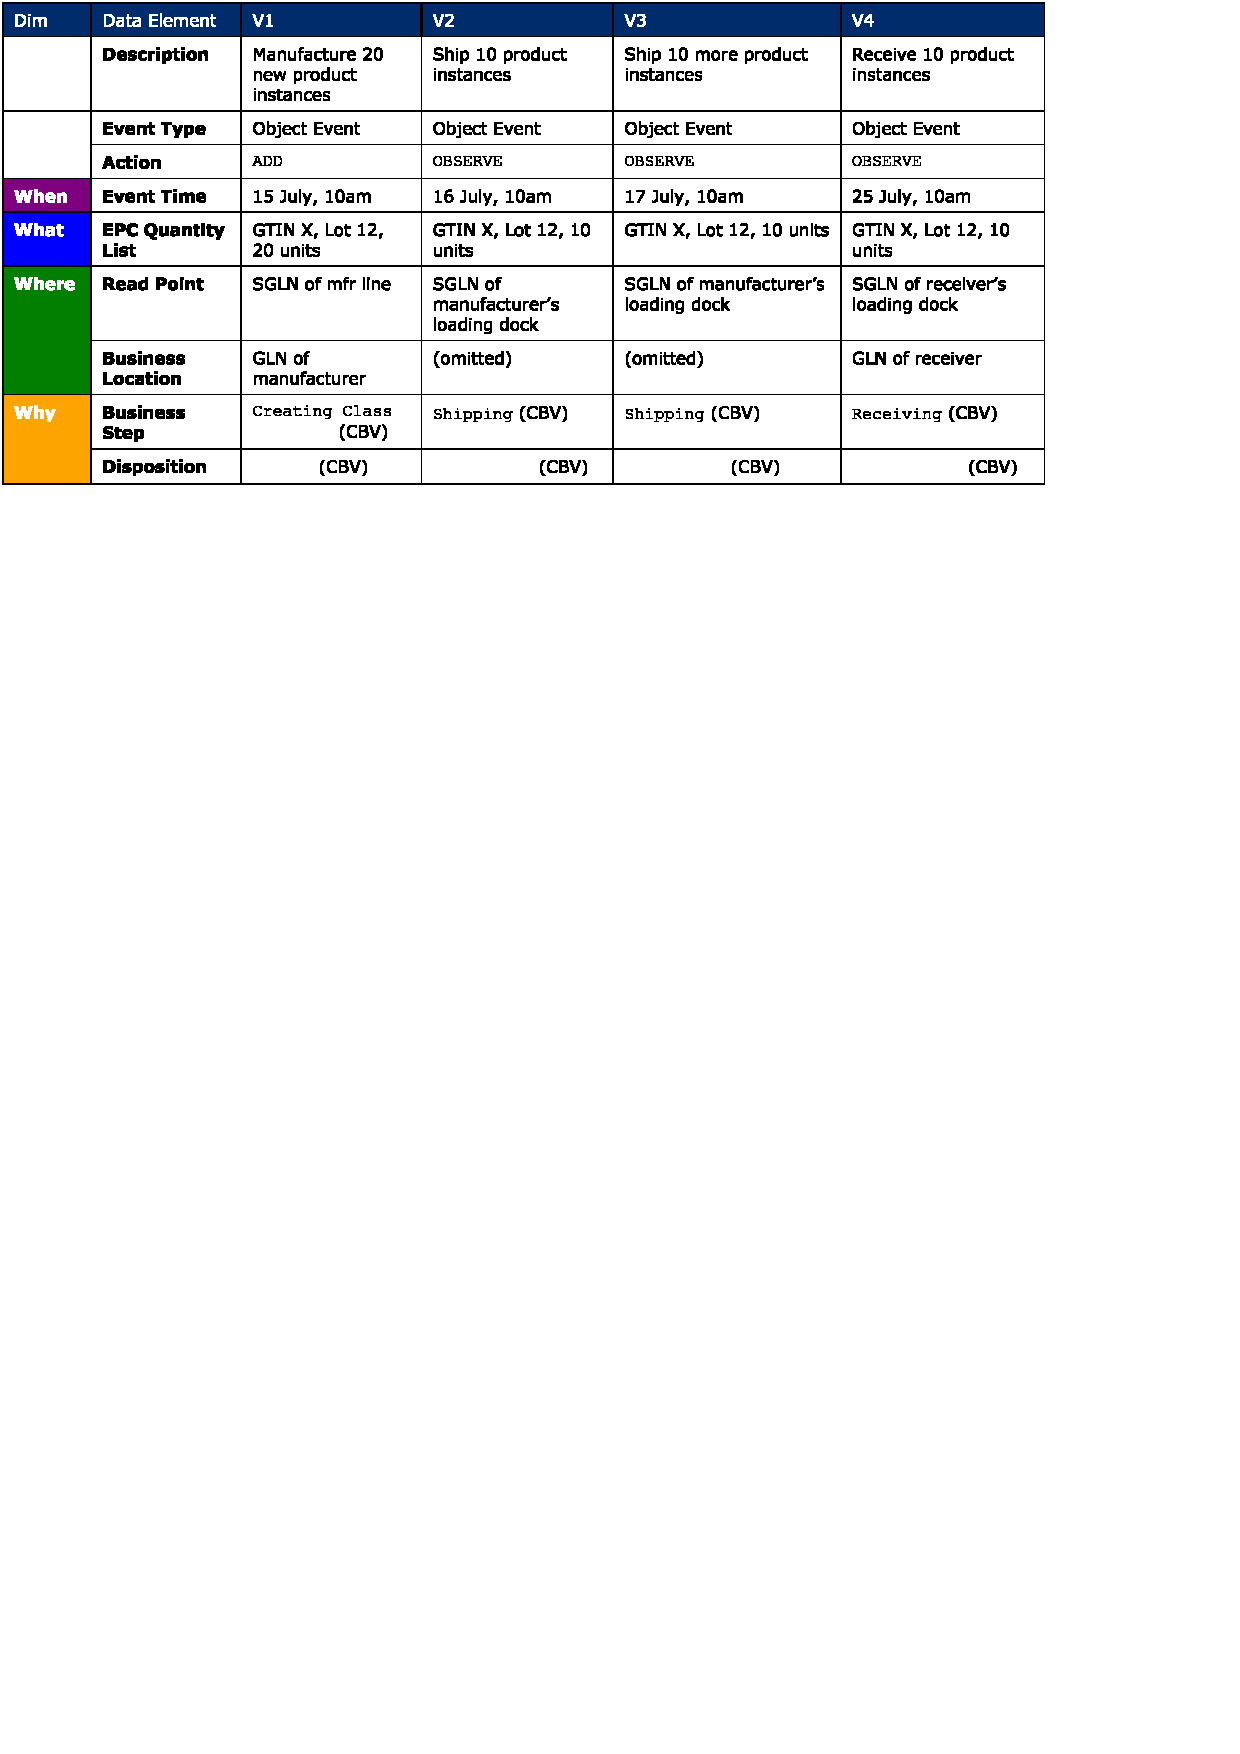
\includegraphics[width=\textwidth]{./figs/02-state-of-the-art/epcis_data_visibility.pdf}
    \caption{\ac{epcis} Event Information Content for \dots of Example Business Process~\cite{EPCISGuidelines}} 
    \label{tab:epciseventinfo}
\end{table}

\subsection{Capture and Query Interfaces}

The \ac{epcis} Data model standardizes the data created and shared across systems. 
To complement the Data model, \ac{epcis} also standardize data interfaces.
\ac{epcis} defines two interfaces: a capture interface, provides means for \ac{epcis}~Events, conforming to the data models, to be saved, typically, in a persistent repository of \ac{epcis} data; and a query interface from which \ac{epcis} data may be requested by applications and trading partners.

The data shared between clients and these interfaces is expressed in \ac{xml} bindings for the data definition models.
The capture interface provides binding that can use either a message queue or \ac{http}. In Code~\ref{code:epcisreport} we can see a \ac{xml} \ac{epcis}~Event example sent to a capture application. 

\begin{listing}
    \inputminted[linenos, breaklines]{xml}{./code/sota/EPCIS_query_response.xml}
    \caption{Example of \ac{epcis}Report sent to a \ac{epcis} capture interface. \ac{epcis} Reports can be extended with User/Vendor Extensions. In this example we see a \texttt{TemperatureC} and \texttt{RelativeHumidity} vendor extension}
    \label{code:epcisreport}
\end{listing}

\ac{epcis} query interface is defined as a web service which can be access by \ac{soap} transport mechanism using the following operations: 

\begin{itemize}
    \item \texttt{poll}: queries for \ac{epcis} events matching specific criteria.
    \item \texttt{subscribe}: allows client to register a subscription for events matching specific criteria, which are delivered asynchronously to the client. 
    \item \texttt{unsubscribe}: removes a registered subscription.
    \item \texttt{getQueryNames}: returns a list with the supported types of queries supported by the service.
    \item \texttt{getSubscriptionIDs}: returns a list of active subscriptions.
    \item \texttt{getStandardVersion}: return the \ac{epcis} version supported by the service.
    \item \texttt{getVendorVersion}: returns a vendor string identifying any non-standard extensions supported by the service (e.g.\ \texttt{TemperatureC} and \texttt{RelativeHumidity} vendor extension in Code~\ref{code:epcisreport})
\end{itemize}

A simple \texttt{poll} operation can be seen in Code~\ref{code:epcisquery}.

\begin{listing}
    \inputminted[linenos, breaklines]{xml}{./code/sota/EPCIS_query.xml}
    \caption{Example of \ac{epcis} Query requesting all \texttt{ObjectEvents} from the Business Location \texttt{urn:epc:id:sgln:76300544.00000.1}}
    \label{code:epcisquery}
\end{listing}

\cleardoublepage